\documentclass[12pt]{article}

\usepackage[utf8]{inputenc}
\usepackage{geometry}
\geometry{
    a4paper,
    total={170mm,257mm},
    left=25mm,
    right=25mm,
    top=25mm,
    bottom=25mm,
}
\usepackage{multicol}
\usepackage[font=small,labelfont=bf]{caption}
\setlength{\columnsep}{0.25cm}
\usepackage[inline]{enumitem}
\usepackage{bm}
\usepackage{amssymb}
\usepackage{xcolor}
\usepackage{mathtools} 
\setlength{\parindent}{0em}
\setlength{\parsep}{0em}
\usepackage{tikz}
\setlength{\parskip}{0em}
\usetikzlibrary{decorations.pathmorphing,patterns}
\usepackage[american,cuteinductors]{circuitikz}
\usetikzlibrary{shapes,arrows,circuits,calc,babel}
% Definition of blocks:
\tikzset{%
  block/.style    = {draw, thick, rectangle, minimum height = 3em,
    minimum width = 3em},
  sum/.style      = {draw, circle, node distance = 2cm}, % Adder
  input/.style    = {coordinate}, % Input
  output/.style   = {coordinate} % Output
}
\usetikzlibrary{shapes.multipart, positioning}
% Defining string as labels of certain blocks.
\newcommand{\suma}{\Large$+$}
\newcommand{\inte}{$\displaystyle \int$}
\newcommand{\derv}{\huge$\frac{d}{dt}$}

\def\mf{\ensuremath\mathbf}
\def\mb{\ensuremath\mathbb}
\def\mc{\ensuremath\mathcal}
\def\lp{\ensuremath\left(}
\def\rp{\ensuremath\right)}
\def\lv{\ensuremath\left\lvert}
\def\rv{\ensuremath\right\rvert}
\def\lV{\ensuremath\left\lVert}
\def\rV{\ensuremath\right\rVert}
\def\lc{\ensuremath\left\{}
\def\rc{\ensuremath\right\}}
\def\ls{\ensuremath\left[}
\def\rs{\ensuremath\right]}
\def\bmx{\ensuremath\begin{bmatrix*}[r]}
\def\emx{\ensuremath\end{bmatrix*}}
\def\bmxc{\ensuremath\begin{bmatrix*}[c]}
\def\emxc{\ensuremath\end{bmatrix*}}
% \def\t{\lp t\rp}
% \def\k{\ls k\rs}

\newcommand{\demoex}[2]{\onslide<#1->\begin{color}{black!60} #2 \end{color}}
\newcommand{\demoexc}[3]{\onslide<#1->\begin{color}{#2} #3 \end{color}}
\newcommand{\anim}[3]{\onslide<#1->{\begin{color}{#2!60} #3 \end{color}}}
\newcommand{\ct}[1]{\lp #1\rp}
\newcommand{\dt}[1]{\ls #1\rs}

% \renewcommand{\familydefault}{\sfdefault}

\begin{document}
\begin{center}
\begin{large}
\textbf{Applied Linear Algebra in Data Analysis}\\
\vspace{0.1cm}
\end{large}
\textbf{Introduction to Optimization}
\end{center}
\hrule
\vspace{1em}

\begin{large}
    \textbf{Marks: 47}
\end{large}


\begin{enumerate}
    \item \textbf{(Feasible sets)} Find and sketch the feasible set for the following optimization problem to minimize $f\ct{\mf{x}}, \, \mf{x} \in \mb{R}^2$, subject to the following constraints. \textbf{[Marks: 5]}
    \begin{enumerate}
        \item $\mf{h}\ct{\mf{x}} = \bmx 3x_1 + 4x_2 - 5 = 0\emx$
        \item $\mf{h}\ct{\mf{x}} = \bmx x_1 - x_2 - 2 = 0\emx^\top$ and $\mf{g}\ct{\mf{x}} = \bmx x_1 + x_2 + 1 \leq 0 \\ x_1 + x_2 - 2 \geq 0 \emx$
        \item $\mf{g}\ct{\mf{x}} = \bmxc x_1 + x_2 \geq 0 \\ x_1 - x_2 \geq 0 \\ \mf{x}^\top\mf{x} \leq 1.0 \\ \mf{x}^\top\mf{x} \geq 0.5\emx$
        \item $\mf{g}\ct{\mf{x}} = \bmxc x_1^2 - x_2 \geq 0 \\ x_1^2 + x_2 + 2 \leq 0 \emx$
        \item $\mf{g}\ct{\mf{x}} = \bmxc -\mf{x}^\top\mf{x} \leq 0 \emx$
    \end{enumerate}

    \item \textbf{(Vector derivatives)} Demonstrate that the following gradients and Hessians with respect to the vector $\mf{x} \in \mb{R}^n$ are true. \textbf{[Marks: 5]}
    \begin{enumerate}
        \item $f\ct{\mf{x}} = \mf{c}^\top \mf{x}$ $\longrightarrow$ $\nabla_{\mf{x}}f\ct{\mf{x}} = \mf{c}^\top$ and $\mf{H}_{f}\ct{\mf{x}} = \mf{0}$
        \item $f\ct{\mf{x}} = \mf{x}^\top\mf{A}\mf{x}$ $\longrightarrow$ $\nabla_{\mf{x}}f\ct{\mf{x}} = 2\mf{x}^\top\mf{A}$ and $\mf{H}_{f}\ct{\mf{x}} = 2\mf{A}$, where $\mf{A}$ is a symmetric matrix.
        \item $f\ct{\mf{x}} = \mf{x}^\top\mf{C}\mf{x}$ $\longrightarrow$ $\nabla_{\mf{x}}f\ct{\mf{x}} = \mf{x}^\top\ct{\mf{C} + \mf{C}^\top}$ and $\mf{H}_{f}\ct{\mf{x}} = \mf{C} + \mf{C}^\top$, where $\mf{C}$ need not be symmetric.
        \item $f\ct{\mf{x}} = \mf{x}^\top\mf{A}\mf{x} + \mf{b}^\top\mf{x} + c$ $\longrightarrow$ $\nabla_{\mf{x}}f\ct{\mf{x}} = 2\mf{x}^\top\mf{A} + \mf{b}^\top$ and $\mf{H}_{f}\ct{\mf{x}} = 2\mf{A}$, where $\mf{A}$ is symmetric.
        \item $\mf{f}\ct{\mf{x}} = \mf{A}\mf{x}$ $\longrightarrow$ $\nabla_{\mf{x}}\mf{f}\ct{\mf{x}} = \mf{A}$.
    \end{enumerate}
    
    \item Does the function $f\ct{\mf{x}} = \mf{c}^\top\mf{x}$, where $\mf{c} \in \mb{R}^n$ have a minimum? Explain your answer. \textbf{[Marks: 1]}
    
    \item Does the function $f\ct{\mf{x}} = \mf{x}^\top\mf{A}\mf{x} + \mf{b}^\top\mf{x} + c$ have a minimum? If so, where is the minimum and explain the conditions under which the function have a minimum. Explain you answer. \textbf{[Marks: 2]}
    
    \item \textbf{(Gradient descent)} Consider function $f: \mb{R} \to \mb{R}$ such that $0 < f''\ct{x} \leq L$ for all $x \in \mb{R}$. Show that the following gradient descent algorithm converges to the minimum of the function $f\ct{x}$.
    \[ x_{k+1} = \mf{x}_k - \alpha_k f'\ct{x_k}, \,\, 0 < \alpha_k < \frac{2}{L}, \, k \in \lc 1, 2, \cdots \rc \]

    This result can be extended to the case of $f: \mb{R}^n \to \mb{R}$, where $0 < \lV\mf{H}_f\ct{\mf{x}}\rV_2 \leq L$ for all $\mf{x} \in \mb{R}^n$. Then, show that the following gradient descent algorithm converges to the minimum of the function $f\ct{\mf{x}}$.\textbf{[Marks: 2]}
    \[ \mf{x}_{k+1} = \mf{x}_k - \alpha_k \nabla f\ct{\mf{x}_k}, \,\, 0 < \alpha_k < \frac{2}{L}, \, k \in \lc 1, 2, \cdots \rc \]
    
    \item \textcolor{blue}{\textbf{[Programming]}} The Rosenbrock's function is given by the following,
    \[ f\ct{\mf{x}} = 100\ct{x_2 - x_1^2}^2 + \ct{1 - x_1}^2 \]
    Write a Python/MATLAB program to minimize the Rosenbrock's function using the following algorithms and terminate the search when the norm of the gradient is less than $10^{-3}$. \textbf{[Marks: 8]}
    \begin{enumerate}
        \item Gradient descent with a fixed step size $\alpha = 0.001$.
        \item Gradient descent with a inexact line search.
        \item Newton's method.
        \item Levenberg-Marquardt method with a $\lambda = 0.1$.
    \end{enumerate}
    Assume $\mf{x}_1 = \bmx -2 & 2\emx^\top$ as the initial guess. Plot the trajectory of the $\mf{x}$ for the four different algorithms in different colors along with the contour of the Rosenbrock's function. How long did the four methods take to reach the termination condition? \textbf{[Marks: 2]}
    
    \item \textbf{(Perceptron)} A perceptron is a simple model of a neuron that takes a set of inputs $\lc x_1, x_2, \ldots, x_n\rc$ and produces an output $y$ based on a set of weights $\lc w_1, w_2, \ldots, w_n\rc$ and a bias $w_0$. The output of the perceptron $y$ is given by the following equation,
    \[ y = f\ct{\sum_{i=1}^n w_i x_i + w_0} \]
    The function $f\ct{\bullet}$ is called the activation function of the perceptron. One of the most common activation functions is the \textit{Sigmoid} function, which is defined as follows,
    \[ f\ct{z} = \frac{1}{1 + \exp\ct{-z}} \]
    The following figure shows a simple perceptron with two inputs $\mf{x} = \bmx x_1 & x_2\emx \in \mb{R}^2$, and a weight vector $\mf{w} = \bmx w_0 & w_1 & w_2 \emx \in \mb{R}^3$. The output of this perceptron is given by,
    \[ y = \frac{1}{1 + \exp\ct{-\mf{w}^\top \bmx 1 \\ \mf{x}\emx}} \]
    % Tikz code for a one input layer (2 neurons), one hidden layer (2 neurons) and one output layer (1 neuron).
    \begin{center}
        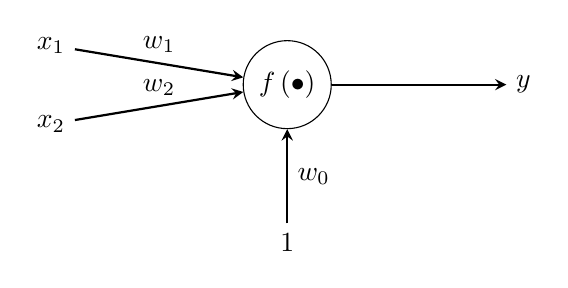
\begin{tikzpicture}[
            % Define the styles for neurons and connections
            neuron/.style={circle, draw, minimum size=1cm},
            connection/.style={-stealth, thick},
            ]
        
            % Number of inputs
            \def\nInputs{2}
        
            % Input Layer
            \foreach \i in {1,...,\nInputs}
                \node[] (I-\i) at (0,-\i) {$x_\i$};
        
            % Perceptron
            \node[neuron] (P) at (3,-1.5) {$f\ct{\bullet}$};
        
            % Output
            \node[] (O) at (6,-1.5) {$y$};
        
            % Bias
            \node[] (B) at (3,-3.5) {$1$};
        
            % Connect inputs to the perceptron
            \foreach \i in {1,...,\nInputs}
                \draw[connection] (I-\i) -- (P) node[midway, above] {$w_\i$};
        
            % Connect bias to the perceptron
            \draw[connection] (B) -- (P) node[midway, right] {$w_0$};
        
            % Connect perceptron to the output
            \draw[connection] (P) -- (O) node[midway, above] {};
        
        \end{tikzpicture}
    \end{center}

    We wish to fit the perceptron to a set of data $\lc\lp \mf{x}_l, y_l \rp\rc_{l=1}^{m}$, where $\mf{x}_l \in \mb{R}^4$ and $y_l \in \lc 0, 1\rc$. The perceptron is trained by minimizing the following loss function,
    \[ l\ct{\mf{w}} = \sum_{l=1}^{m} \lp y_l - \frac{1}{1 + \exp\ct{-\mf{w}^\top \tilde{\mf{x}}_i}}\rp^2 \]
    where, $\tilde{\mf{x}}_i = \bmxc 1 \\ \mf{x}_l\emx$.

    The optimization problem can be formulated as the following,
    \[ \mf{w}^* = \arg\min_{\mf{w}} l\ct{\mf{w}} \]

    We can solve this using a gradient descent algorithm, starting with a random guess for the weight vector $\mf{w}_1$ and update the weight vector using the following update rule,
    \[ \mf{w}_{k+1} = \mf{w}_k - \alpha_k \nabla l\ct{\mf{w}_k} \]
    where, $\alpha_k$ is the step size. 
    
    Find the expression for the gradient of the loss function $\nabla l\ct{\mf{w}}$. \textbf{[Marks: 4]}

    \item Consider the following optimization problem,
    \[  \begin{split}
        \min_{\mf{x}} &\,\, \frac{1}{2}\mf{x}^\top\mf{Q}\mf{x} \\
        \text{s.t. } &\,\, \mf{x}^\top\mf{P}\mf{x} = 1
       \end{split} \]
    Find the expression for the minimizer of this problem $\mf{x}^*$ and the minimum value of the objective function $\frac{1}{2}\mf{x}^\top\mf{Q}\mf{x}$. \textbf{[Marks: 2]}
       
    \item Find the minimizer and maximizer of the following optimization problem $\mf{x} \in \mb{R}^3$,
    \[  \begin{split}
        \min_{\mf{x}} &\,\, \ct{\mf{a}^\top \mf{x}}\ct{\mf{b}^\top \mf{x}} \\
        \text{s.t. } &\,\, x_1 + x_2 = 0\\
                    &\,\, x_2 + x_3 = 0
        \end{split} \]
    where, $\mf{a} = \bmx 0 \\ 1 \\ 0\emx$ and $\mf{b} = \bmx 1 \\ 0 \\ 1\emx$. \textbf{[Marks: 2]}
        
    \item Consider the following optimization problem,
    \[  \begin{split}
        \min_{\mf{x}} &\,\, \ct{x_1 - a}^2 + \ct{x_2 - b}^2 \\
        \text{s.t. } &\,\, x_1^2 + x_2^2 \leq 1
        \end{split} \]
    where, $a, b \in \mb{R}$ are constant such that $a^2 + b^2 \geq 1$.
    
    Let $\mf{x}^* = \bmx x_1^* & x_2^*\emx^\top$ be the minimizer of the above optimization problem.  \textbf{[Marks: 10]}
    \begin{enumerate}
        \item Use the first order necessary conditions for the unconstrained optimization problem to show that $\ct{x_1^*}^2 + \ct{x_2^*}^2 = 1$.
        \item Use the KKT theorem to show that $\mf{x}^*$ is unique and has the form $\mf{x}^* = \alpha\bmx a \\ b\emx$, where $\alpha \in \mb{R}$ is a positive constant.
        \item Find the expression for $\alpha$ in terms of $a$ and $b$.
        \item Can you explain the solution to this problem geometrically.
        \item Does the above analysis hold when the constraint $a^2 + b^2 < 1$? Explain your answer. If it does not, what would be the solution $\mf{x}^*$ in this case?
    \end{enumerate}
    
    \item Consider the following optimization problem,
    \[  \begin{split}
        \min_{\mf{x}} &\,\, \mf{c}^\top\mf{x} \\
        \text{s.t. } &\,\, \mf{a}^\top \mf{x} \leq b
        \end{split} \]
    where, the non-zero vectors $\mf{a}, \mf{c} \in \mb{R}^n$ and $b \in \mb{R}$ are constants.  \textbf{[Marks: 6]}
    \begin{enumerate}
        \item Under what conditions does the above optimization problem have a solution?
        \item When the above optimization problem has a solution, is the solution unique? If yes, find the unique minimizer $\mf{x}^*$, else find the set of all minimizers.
        \item Can you explain these results geometrically?
    \end{enumerate}
\end{enumerate}
\end{document}